\documentclass[oneside,a4paper,14pt]{extarticle}
\usepackage[a4paper,letterpaper,top=20mm,bottom=20mm,left=20mm,right=10mm]{geometry}
\usepackage[russian]{babel}
\usepackage{indentfirst}
\usepackage{graphicx}
\usepackage{caption}
\usepackage{titlesec}
\usepackage{minted, fancyvrb}
\usepackage{hyperref}
\usepackage{enumitem}
\usepackage{amsmath}
\usepackage{fancyhdr}
\usepackage{colortbl}
\usepackage[dvipsnames]{xcolor}
\usepackage{float}

\setminted{style = rainbow_dash, fontsize = \small}

\titleformat{\section}{\normalsize\bfseries}{\thesection}{1em}{}
\titleformat{\subsection}{\normalsize\bfseries}{\thesubsection}{1em}{}
\titleformat{\subsubsection}{\normalsize\bfseries}{\thesubsubsection}{1em}{}

\renewcommand\baselinestretch{1.33}
\setlength{\parindent}{1.25cm}

\setlist[enumerate]{
  left=0.5\parindent,
  label=\arabic*.,
  itemsep=0pt,
  topsep=5pt,
  partopsep=0pt,
  parsep=0pt
}
\setlist[itemize]{
  left=0.5\parindent,
  itemsep=0pt,
  topsep=5pt,
  partopsep=0pt,
  parsep=0pt
}

\hypersetup{
  colorlinks=true,
  linkcolor=black,
  urlcolor=blue,
  pdfborder={0 0 0},
  pdftitle={Построение 7-битного счётчика с переменным коэффициентом пересчёта},
  pdfauthor={Черкасов А.А. и Зинин В.А.},
}

\begin{document}

\newpage
\thispagestyle{empty}
\begin{center}
  МИНИСТЕРСТВО НАУКИ И ВЫСШЕГО ОБРАЗОВАНИЯ РОССИЙСКОЙ ФЕДЕРАЦИИ\\
  ФЕДЕРАЛЬНОЕ ГОСУДАРСТВЕННОЕ БЮДЖЕТНОЕ УЧРЕЖДЕНИЕ ВЫСШЕГО ОБРАЗОВАНИЯ\\
  <<ВЯТСКИЙ ГОСУДАРСТВЕННЫЙ УНИВЕРСИТЕТ>>\\
  Институт математики и информационных систем\\
  Факультет автоматики и вычислительной техники\\
  Кафедра электронных вычислительных машин
\end{center}
\vspace{10mm}

\hfill
\begin{tabular}{l}
  \footnotesize Дата сдачи на проверку:                                          \\
  \footnotesize <<\rule[-1mm]{5mm}{0.10mm}\/>>\rule[-1mm]{20mm}{0.10mm}\ 2025 г. \\
  \footnotesize Проверено:                                                       \\
  \footnotesize <<\rule[-1mm]{5mm}{0.10mm}\/>>\rule[-1mm]{20mm}{0.10mm}\ 2025 г. \\
\end{tabular}
\vfill

\begin{center}
  Отчёт по лабораторной работе №4\\
  по дисциплине\\
  <<Цифровая схемотехника>>\\
  \textbf{Построение 7-битного счётчика с переменным коэффициентом пересчёта}\\
\end{center}
\vspace{25mm}
\noindent
\begin{tabular}{ll}
  Разработали студенты гр. ИВТб-2301-05-00 & \hspace{5mm}\rule[-1mm]{30mm}{0.10mm}\,/Черкасов А. А./ \\
                                           & \hspace{5mm}\rule[-1mm]{30mm}{0.10mm}\,/Зинин В. А./    \\
                                           & \hspace{12.5mm}\footnotesize(подпись)                   \\
  Преподаватель                           & \hspace{5mm}\rule[-1mm]{30mm}{0.10mm}\,/Мельцов В. Ю./  \\
                                           & \hspace{12.5mm}\footnotesize(подпись)                   \\
\end{tabular}

\noindent
\begin{tabular}{lp{58mm}r}
  Работа защищена &  & \hspace{5mm}<<\rule[-1mm]{5mm}{0.10mm}\/>>\rule[-1mm]{30mm}{0.10mm}\ 2026 г.
\end{tabular}
\vfill

\begin{center}
  Киров\\
  2026
\end{center}

\newpage\thispagestyle{plain}

\section{Цель лабораторной работы}
Получить навыки построения и анализа 7-битного счётчика с коэффициентом пересчёта 103. Изучить принцип программирования коэффициента деления с помощью логических элементов на базе микросхем ЛА3, ЛА4, ЛН1, ИЕ7, ТМ2 (серия ТТЛ).

\section{Теоретическое описание}
\subsection{Двоичный счётчик ИЕ7}
Микросхема К155ИЕ7 представляет собой 4-битный синхронный двоичный счётчик с предустановкой. Имеет входы предустановки данных $D_0\ldots D_3$, вход синхронизации $C$, вход сброса $R$, вход разрешения записи $WR$ и выходы $Q_0\ldots Q_3$. Счётчик переключается по спаду тактового импульса.

\subsection{Программируемый коэффициент пересчёта}
Для получения требуемого коэффициента деления используется метод предустановки (parallel load). Два счётчика ИЕ7 образуют 8-битный счётчик, из которого задействовано 7 бит. При достижении кода, соответствующего коэффициенту 103, на выходах счётчика с помощью логических элементов (ЛА3, ЛА4, ЛН1) формируется сигнал загрузки, который записывает начальное значение, и цикл счёта повторяется. Таким образом, коэффициент пересчёта составляет 103.

\subsection{D-триггер ТМ2}
Микросхема К155ТМ2 содержит два D-триггера. В работе используется один триггер для дополнительной синхронизации и формирования выходных сигналов.

\section{Функциональная схема счётчика}
На рисунке 1 представлена функциональная схема 7-битного счётчика с переменным коэффициентом пересчёта. Два счётчика ИЕ7 включены последовательно, образуя 8-битный счётчик, из которого используется 7 бит. Логические элементы ЛА3, ЛА4 формируют сигнал сброса/загрузки при достижении заданного кода.

\begin{figure}[H]
  \centering
  
\includegraphics[width=0.9\textwidth]{pics/functional_diagram.png}
  \caption*{Рисунок 1 --- Функциональная схема 7-битного счётчика с коэффициентом пересчёта 103}
\end{figure}

\section{Принципиальная схема устройства}
Принципиальная схема (рисунок 2) выполнена на микросхемах серии ТТЛ: \textbf{ЛА3} (4 элемента 2И-НЕ), \textbf{ЛА4} (3 элемента 3И-НЕ), \textbf{ЛН1} (6 инверторов), \textbf{ИЕ7} (два 4-битных двоичных счётчика) и \textbf{ТМ2} (один D-триггер). Логические элементы формируют сигнал управления предустановкой для задания коэффициента пересчёта 103. Схема включения микросхем соответствует заводским цоколёвкам. Питание подаётся от источника +5~В.

\begin{figure}[H]
  \centering
  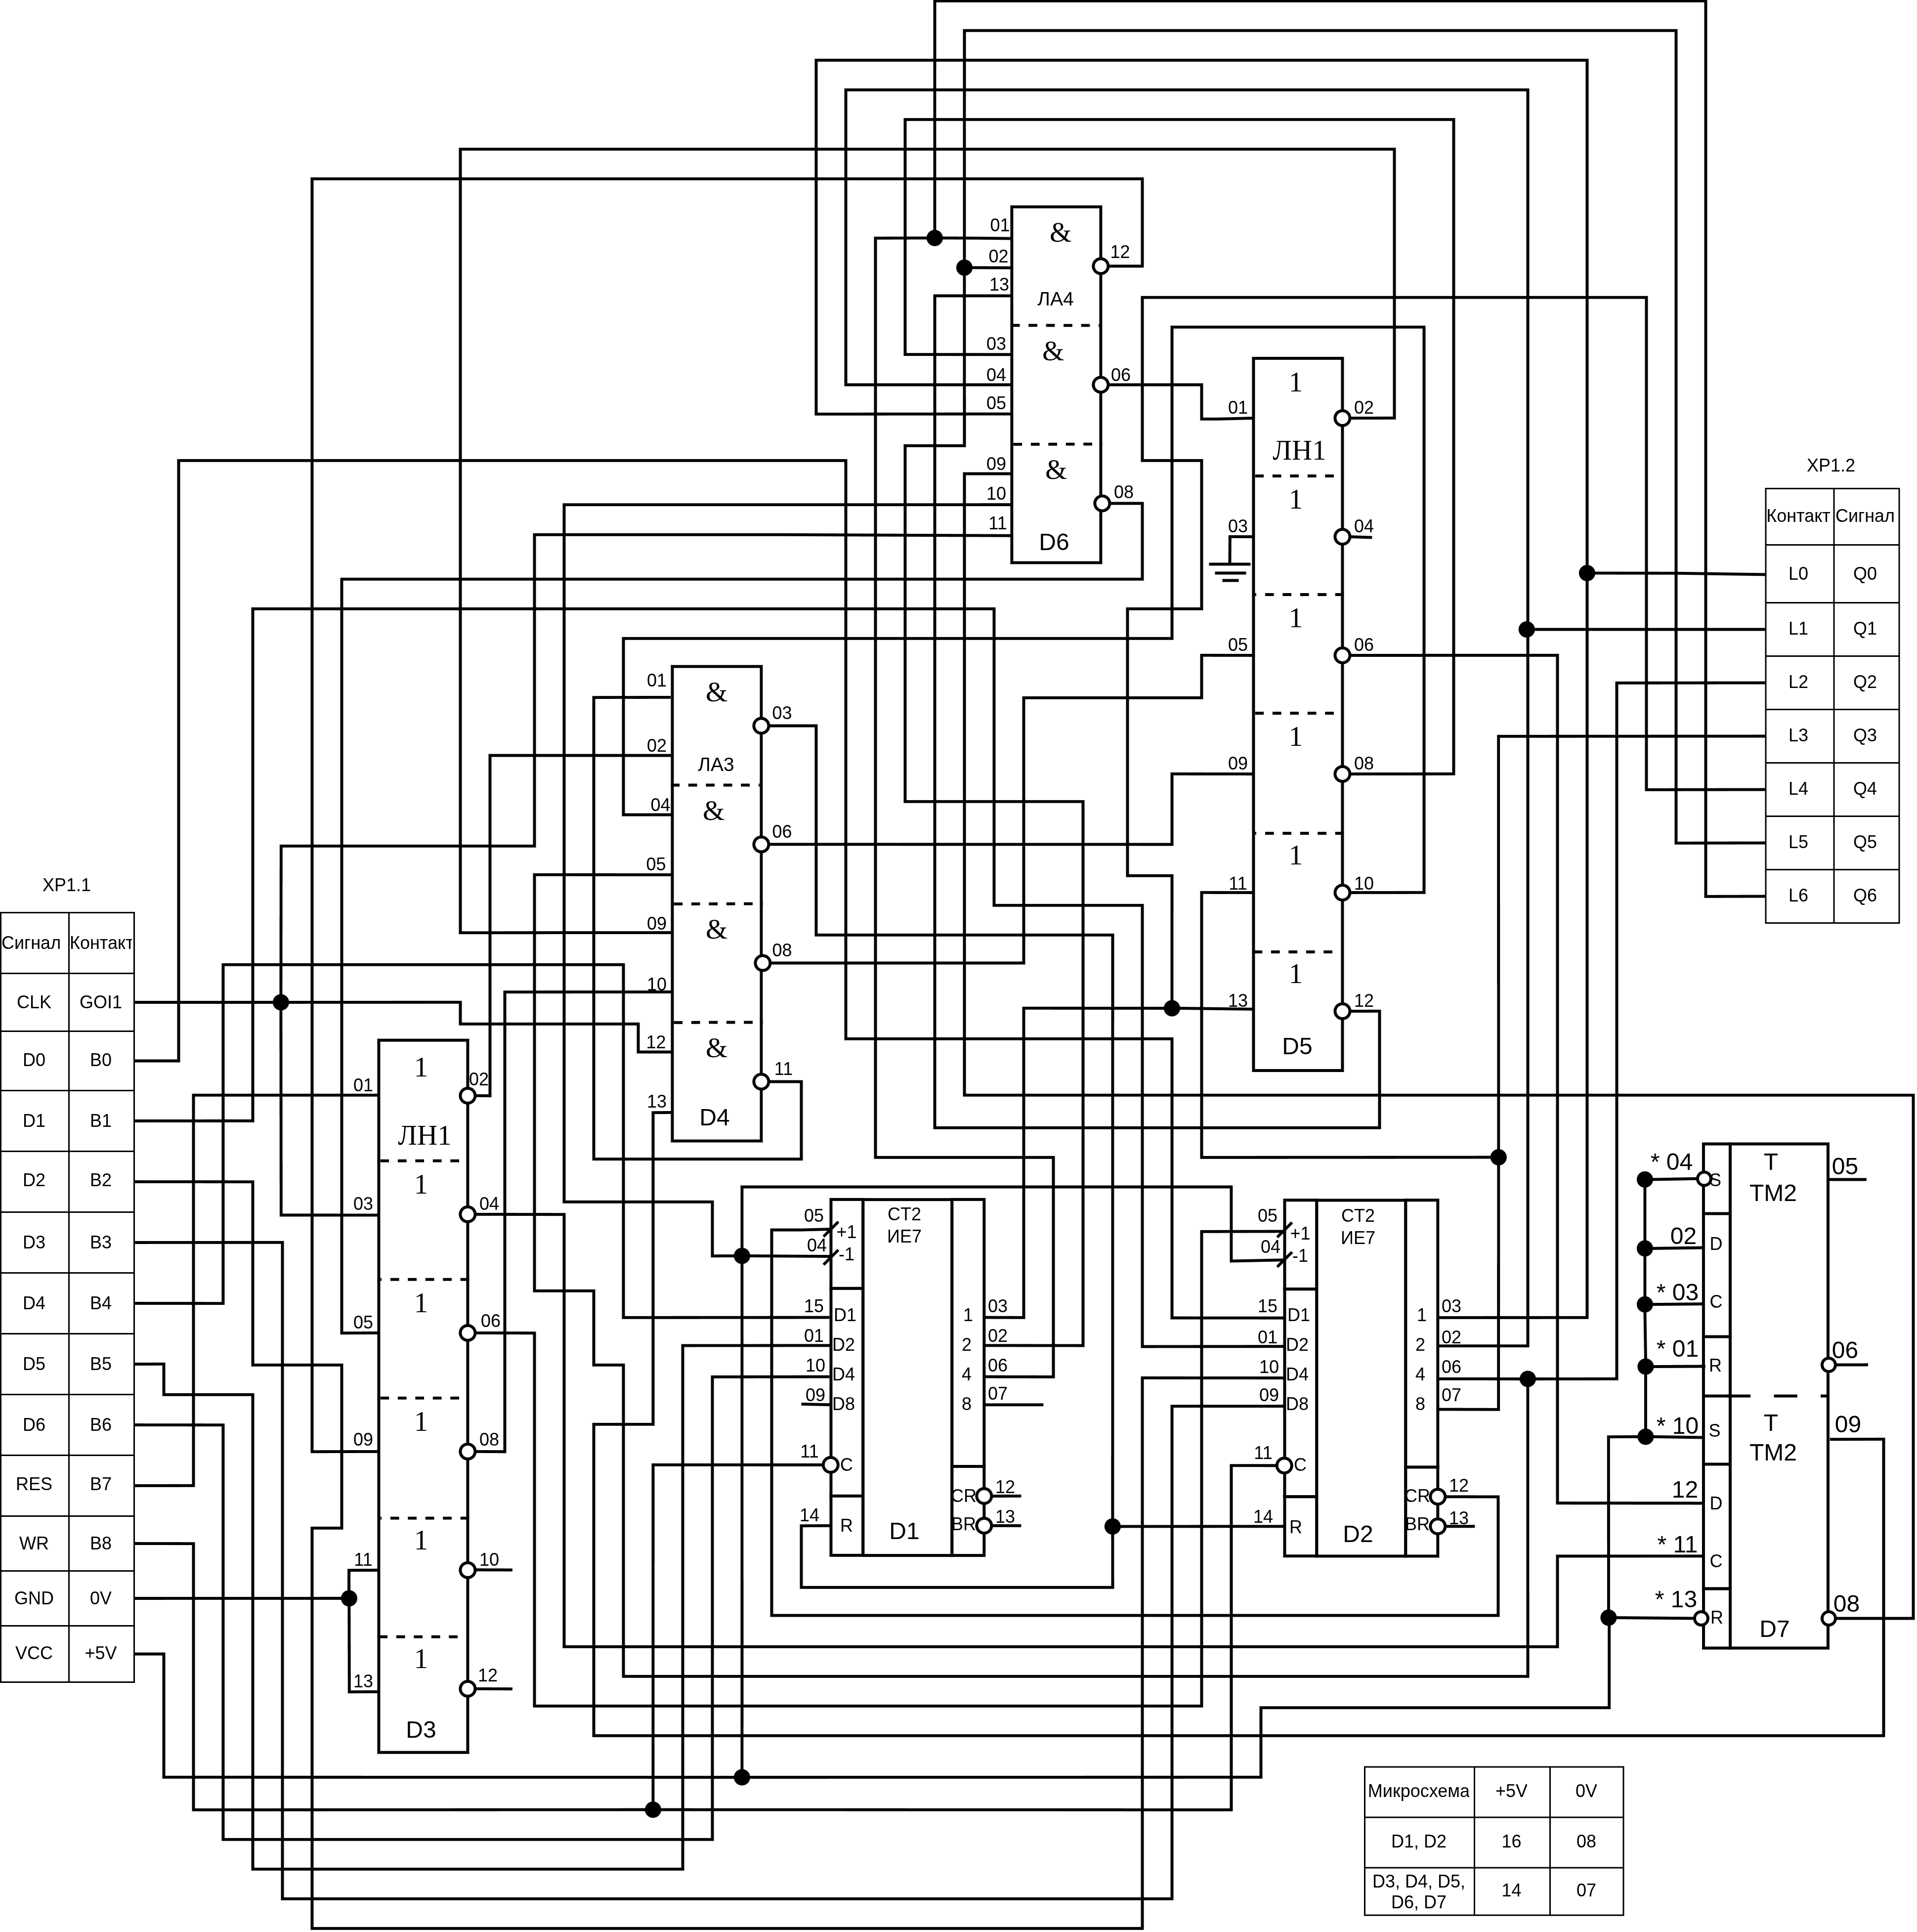
\includegraphics[width=0.95\textwidth]{pics/principle_diagram.png}
  \caption*{Рисунок 2 --- Принципиальная схема 7-битного счётчика с коэффициентом пересчёта 103}
\end{figure}

\section*{Вывод}
В ходе лабораторной работы были получены практические навыки построения 7-битного счётчика с переменным коэффициентом пересчёта. Счётчик реализован на базе двух микросхем ИЕ7, логических элементов ЛА3, ЛА4, ЛН1 и D-триггера ТМ2. Разработаны функциональная и принципиальная схемы устройства. Полученные результаты могут быть использованы при проектировании делителей частоты с произвольным коэффициентом деления в цифровых устройствах.

\end{document}
